\documentclass[12pt]{article}
\usepackage{amsmath, amssymb, graphicx, hyperref, geometry, booktabs, longtable}
\geometry{margin=1in}
\setlength{\parindent}{0pt} % Removes paragraph indentation

\title{\Huge \textbf{The Impact of Travel and Schedule Density on Player Performance in the NBA}\\
\LARGE Insights from Statistical and Logistic Regression}
\author{
  Aamogh Sawant, 
  Nathan Wright
}
\date{September 25, 2024}

\begin{document}
\maketitle

\newpage
\tableofcontents
\newpage

\section{Abstract}
The schedules that professional athletes usually are bound by are quite tight and involve a lot of traveling, which in turn might affect performances and health. With the NBA, factors like travel distance, time zone shifts, and game density (back-to-back games, for example) become very important in determining player efficiency and overall team success. This paper investigates the quantitative effects of travel and schedule density on various indicators of player performance, such as shooting efficiency, defensive effectiveness, and turnover rates, by using historical data with both statistical and machine learning approaches. Our findings are meant to provide actionable insights to teams in order to optimize player workload, enhance performances, and reduce the chance of injury. We will also discuss more general implications of this work in other sports and health contexts.

\section{Introduction}
Travel and schedule density are critical yet understudied factors affecting performance in professional sports. The NBA, with its grueling schedule, offers a unique environment to examine these effects. Frequent travel and long road trips, along with game schedules that are condensed, could potentially cause fatigue, decreased efficiency, and a higher rate of injury among players.

This study investigates the impact of travel demands and game congestion on player performance indicators. It quantifies the extent to which factors such as travel distances, time zone changes, and consecutive games impact key performance indicators like shooting percentages, defensive performances, and turnover rates. Additionally, it considers situational elements like performance disparity between home and away games, rest days, and opponent strength in order to provide a comprehensive analysis.

The main goal is to provide tangible recommendations that support teams in improving player workload management and decreasing the risk of injuries. Besides, the study looks at the opportunities to extend this study to cover other sports and its applicability to business analytics.


\section{Related Research}
The impact of travel and scheduling on athletic performance is well-studied area in the domain of sports science. One of the main focuses of this research has been the disruption of circadian rhythms due to crossing multiple time zones, leading to the condition known as jet lag. Research by Chtourou and Souissi (2012) shows athletes crossing more than two time zones to have decreases in reaction time, endurance, and strength, mainly during the first 48 hours after arrival. This is very relevant to the NBA, as teams tend to travel across time zones, thus impacting performance, most notably in away games.

Further research highlights adverse effects that extended road trips have on teams, which contribute to fatigue resulting from continuous travel and not enough sleep with less recovery time. Dall'Acqua et al. (2014) reported significant decreases in shooting accuracy during extended road trips especially if games are back to back. It was further recorded by Ferkins et al. (2011) that defensive performances also suffer during away matches due to accumulated fatigue, this increases fouls and defensive lapses. Similarly, Bessone et al. (2018) associated frequent travel, especially back-to-back games, with higher turnover rates since players' focus wanes when tired.

Recent studies using machine-learning approaches, such as Lee and Lee (2020), have explored the impact of travel on athlete performance. Their findings suggested that increased travel load negatively impacted shooting percentages and assist-to-turnover ratios, which may suggest improved scheduling to optimize performance outcomes. The study by Weschler et al. (2019) has also shown that experienced players are less affected by the fatigue from travel, stressing the variation in how different athletes cope with travel-related stress.

This paper uses both statistical and machine-learning approaches to build on the findings of the impact of travel and scheduling on NBA player performance. We incorporate variables such as time zone changes, consecutive game sets, and rest days to provide actionable suggestions for optimizing team scheduling.

\section{Methods}
To analyze the relationship between travel and NBA team performance, a combination of geospatial analysis, statistical modeling, and data visualization was employed. This methodology integrates travel data with team performance metrics to uncover actionable insights into the effects of travel distances on team efficiency during the 2018 NBA season.

\subsection{Travel Data Calculation}
Travel distances between NBA cities were computed using geographical coordinates with the \texttt{geopy.distance} library, which calculates great-circle distances between two points on the Earth’s surface. Using these distances, flight times were estimated assuming an average flight speed of 805 kilometers per hour (500 miles per hour). A comprehensive pairwise travel matrix was generated, accounting for all NBA cities. Adjustments were made for cases where travel time was negligible, such as games between teams located in the same city (e.g., LA Lakers and LA Clippers, New York Knicks and Brooklyn Nets), where travel times were set to zero.

The resulting travel data was exported as a CSV file for integration with game performance data.

\subsection{Performance Metrics and Data Preprocessing}
Game-level data, including team and opponent statistics, was sourced and filtered for games during the 2018 NBA season. Preprocessing steps included:
\begin{itemize}
    \item \textbf{Date Standardization:} Game dates were converted to a uniform \texttt{datetime} format to enable temporal filtering.
    \item \textbf{Filtering Games:} Home games and games with zero travel distance were excluded to focus on the effects of travel.
    \item \textbf{Derived Metrics:} Key performance metrics were calculated:
    \begin{itemize}
        \item \textit{Offensive Rating (OffRtg):} Points scored per 100 field goal attempts.
        \item \textit{Defensive Rating (DefRtg):} Opponent points allowed per 100 opponent field goal attempts.
        \item \textit{Rating Differential (Rating\_Diff):} The difference between OffRtg and DefRtg, reflecting overall team efficiency.
    \end{itemize}
\end{itemize}

\subsection{Statistical Modeling}
To investigate the impact of travel on team performance, linear regression models were employed:
\begin{itemize}
    \item \textbf{Independent Variable:} Travel distance (measured in flight time, in minutes).
    \item \textbf{Dependent Variable:} Offensive-to-Defensive Rating Ratio (\texttt{OffDef\_Ratio}), representing the relative efficiency of a team in offense compared to defense.
\end{itemize}


For team-specific insights, regression analyses were performed for each NBA team individually. A combined regression analysis was conducted across all teams to identify league-wide trends. The Ordinary Least Squares (OLS) regression method was utilized, with statistical metrics such as R-squared values and p-values evaluated to determine the strength and significance of the relationships.

\subsection{Visualization and Insights}
Scatter plots were generated to illustrate the relationship between travel distance and the Offensive-to-Defensive Rating Ratio for individual teams, with regression lines superimposed to highlight trends. A combined scatter plot, encompassing data from all teams in 2018, was created to visualize league-wide patterns. These visualizations were created using the \texttt{seaborn} library, ensuring clarity and readability. The scatter plots provide insights into how travel distance impacts team performance, with regression lines showing the direction and strength of these relationships.
\begin{figure}[h!]
    \centering
    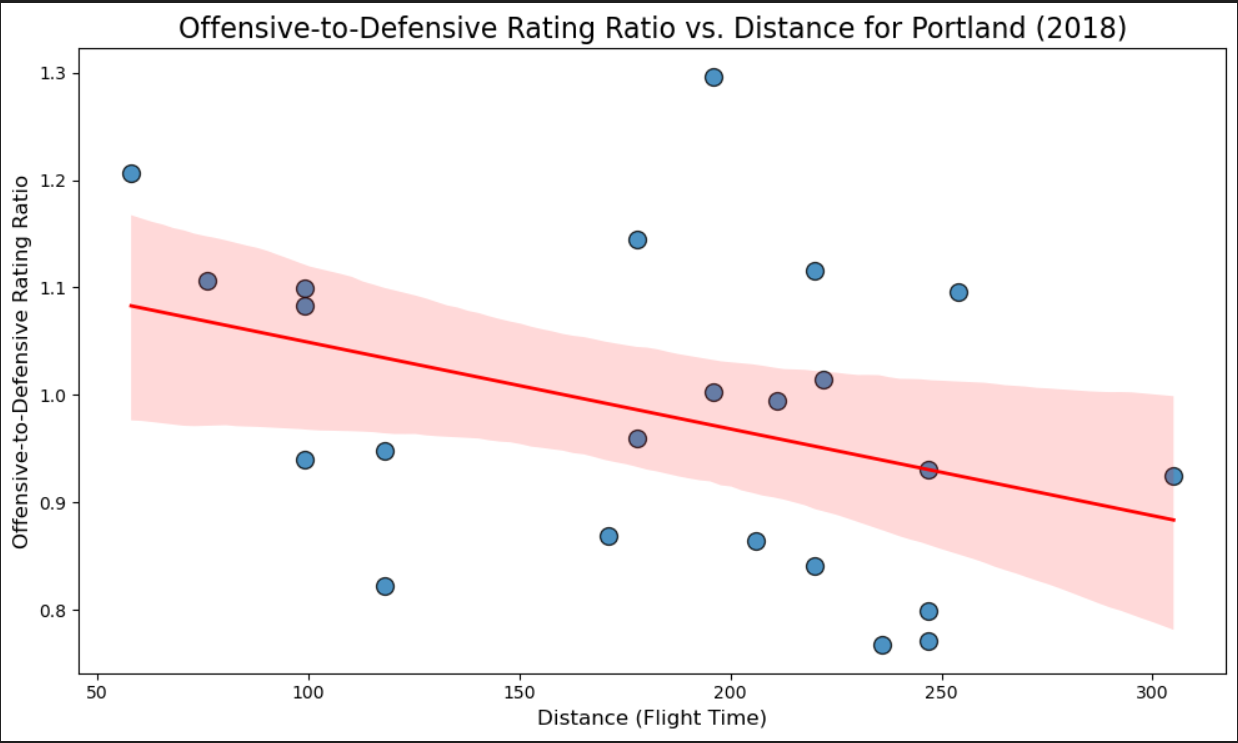
\includegraphics[width=0.8\textwidth]{Screenshot 2024-12-18 131654.png}
    \caption{Scatter plot of travel distance versus team performance (OffDef\_Ratio) for Portland.}
    \label{fig:travel_performance_portland}
\end{figure}
\begin{figure}[h!]
    \centering
    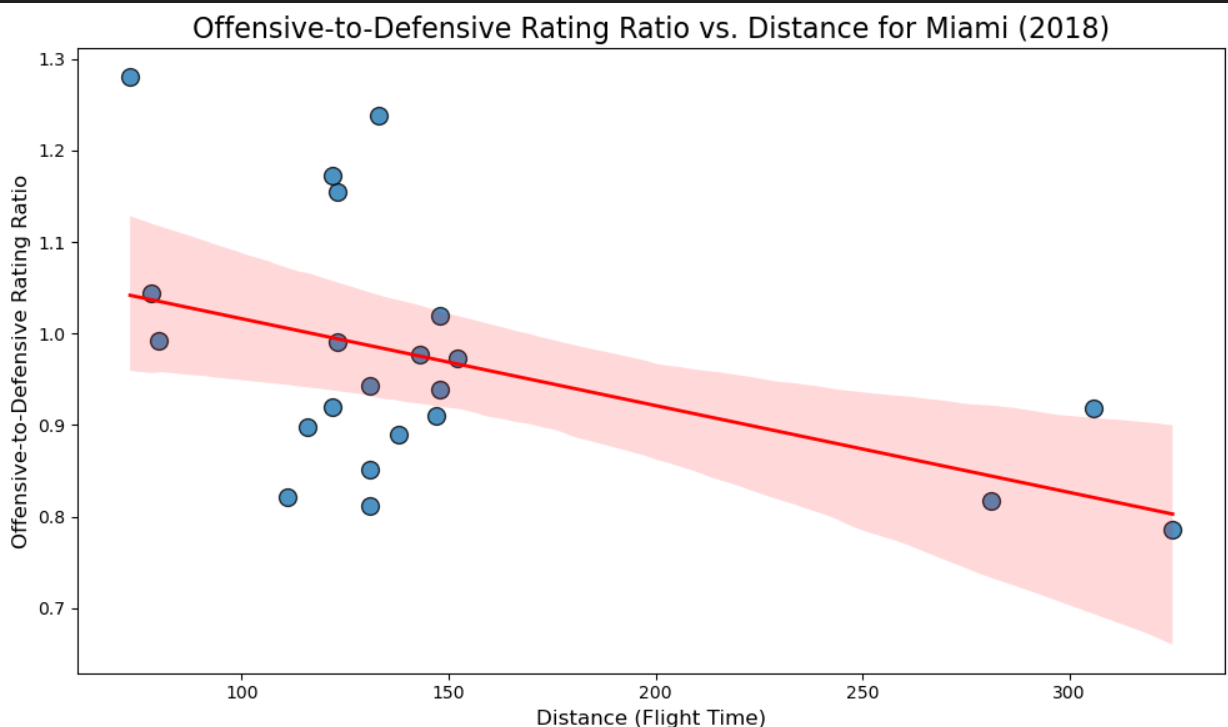
\includegraphics[width=0.8\textwidth]{Screenshot 2024-12-18 142519.png}
    \caption{Scatter plot of travel distance versus team performance (OffDef\_Ratio) for Miami.}
    \label{fig:travel_performance_laclippers2}
\end{figure}
\begin{figure}[h!]
    \centering
    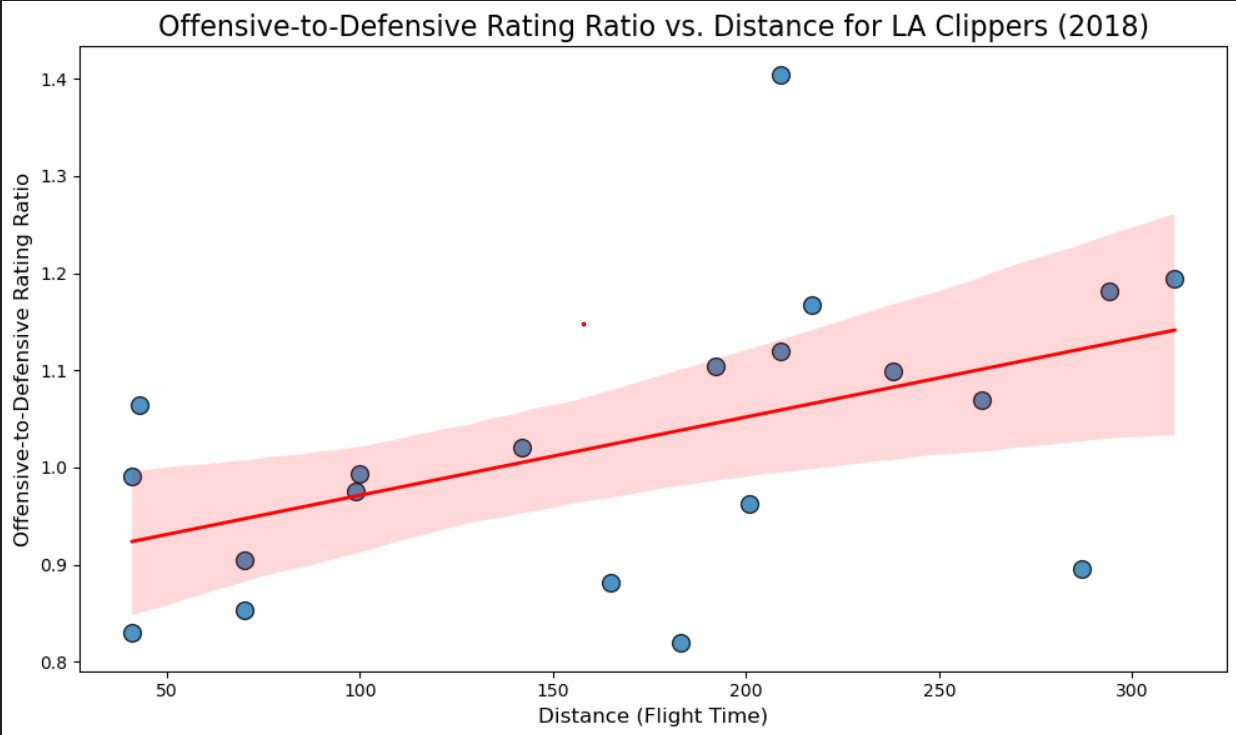
\includegraphics[width=0.8\textwidth]{Screenshot 2024-12-18 141637.png}
    \caption{Scatter plot of travel distance versus team performance (OffDef\_Ratio) for LA Clippers.}
    \label{fig:travel_performance_laclippers1}
\end{figure}
\begin{figure}[h!]
    \centering
    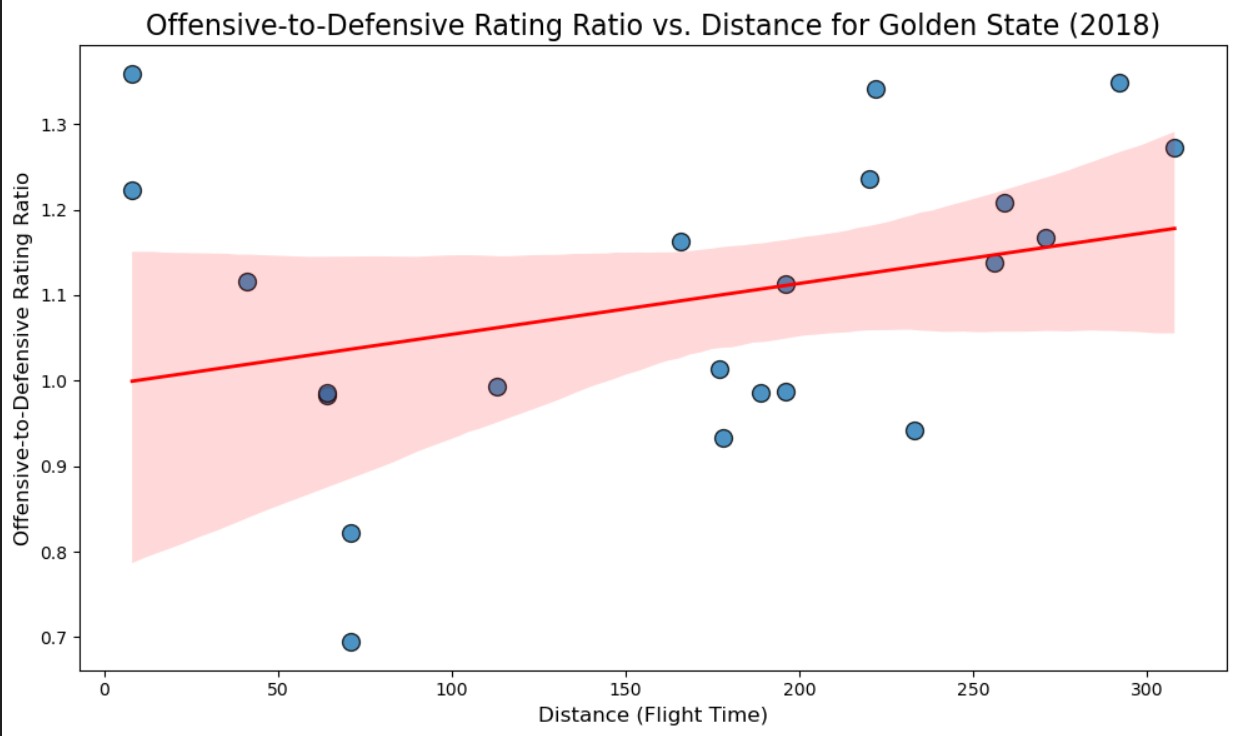
\includegraphics[width=0.8\textwidth]{Screenshot 2024-12-18 142937.png}
    \caption{Scatter plot of travel distance versus team performance (OffDef\_Ratio) for Golden State Warriors.}
    \label{fig:travel_performance_laclippers1}
\end{figure}

\begin{figure}[h!]
    \centering
    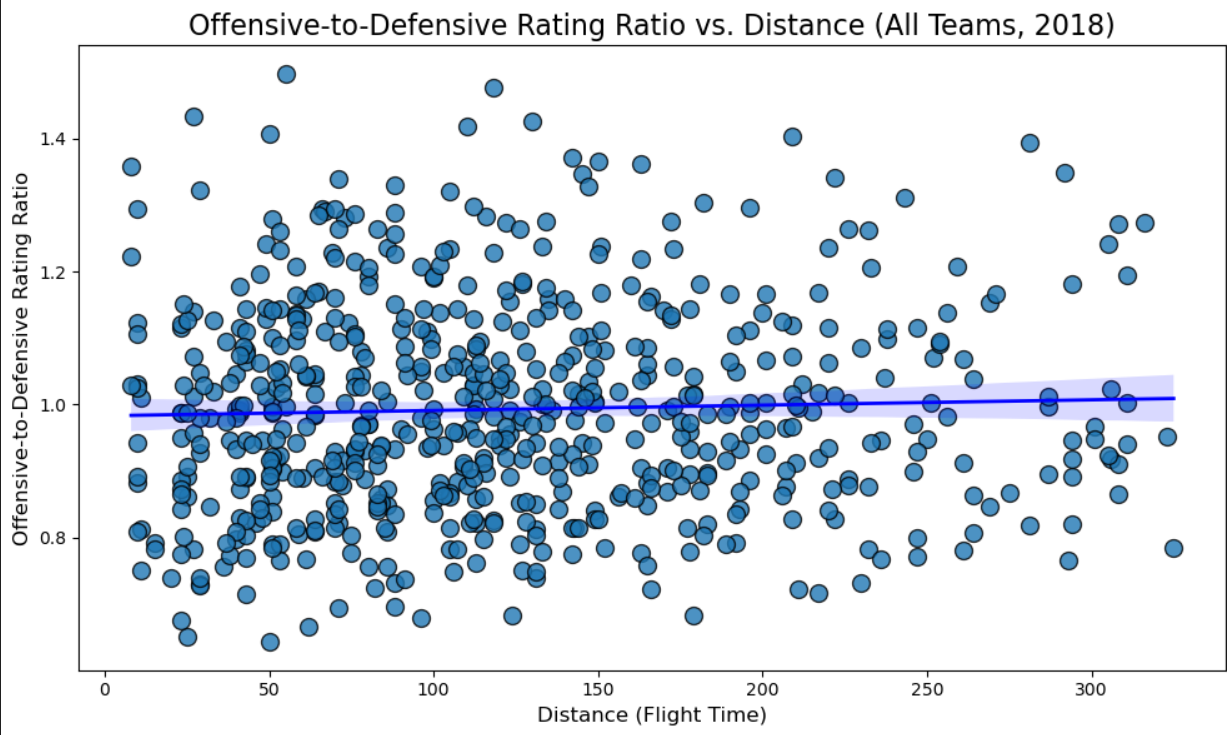
\includegraphics[width=0.8\textwidth]{Screenshot 2024-12-18 144058.png}
    \caption{Scatter plot of travel distance versus team performance (OffDef\_Ratio) for Overall League.}
    \label{fig:travel_performance_laclippers1}
\end{figure}

\clearpage
\subsection{Validation}
The reliability of the statistical models was validated through a series of iterative tests and parameter adjustments, using metrics such as R-squared values to measure model fit and p-values to determine the statistical significance of travel distance as a predictor of team performance. This expansive framework showed the effects of travel on NBA team performance during the 2018 season on both an individual and league-wide basis.

\subsection{League-Wide Analysis}
At the league level, the analysis revealed mixed relationships between travel distance and team performance, measured by the Offensive-to-Defensive Rating Ratio (\texttt{Rating\_Diff}). Pearson correlation coefficients computed for all teams demonstrated variability in how travel distance related to performance:

\subsubsection*{Positive Correlations}
Several teams exhibited positive correlations between travel distance and performance:
\begin{itemize}
    \item \textbf{LA Clippers (0.4843), Golden State Warriors (0.3203), Sacramento Kings (0.4650), and Toronto Raptors (0.4780)}: These teams, on average, performed better with increased travel distance. Possible factors include efficient travel arrangements, strong roster depth, and mental preparedness for away games.
\end{itemize}

\subsubsection*{Negative Correlations}
Conversely, other teams showed significant negative correlations:
\begin{itemize}
    \item \textbf{Miami Heat (-0.4675), Portland Trail Blazers (-0.3751), and Houston Rockets (-0.2603)}: For these teams, longer travel distances seemed to hinder performance, potentially due to fatigue, routine disruptions, or recovery inefficiencies.
\end{itemize}

\subsubsection*{Marginal Correlations}
A few teams displayed negligible correlations, indicating little to no perceivable effect of travel distance on performance:
\begin{itemize}
    \item \textbf{Chicago Bulls (0.0204) and Denver Nuggets (-0.0510)}: These teams exhibited correlations approximately equal to zero.
\end{itemize}

The variation in correlations across teams highlights the complex nature of the travel-performance relationship in the NBA. Factors such as team travel schedules, geographical location, recovery strategies, and mental resilience likely contribute to these differences.

\subsection{Team-Specific Analysis}

\subsubsection*{LA Clippers}
The LA Clippers showed a strong positive correlation of 0.4843, indicating that their performance improved with increased travel distances. This suggests that the Clippers effectively managed travel-related strains, potentially through strong recovery strategies or enhanced focus during away games. A scatter plot of their \texttt{Rating\_Diff} showed an upward trend, emphasizing their ability to adapt to varying travel conditions.

\subsubsection*{Golden State Warriors}
The Golden State Warriors exhibited a positive correlation of 0.3203, reflecting improved performance with longer travel distances. This may be attributed to their deep roster, strong leadership, and experience in handling travel demands. A regression analysis of their performance showed a moderate upward trend, reinforcing their resilience during the 2018 season.

\subsubsection*{Miami Heat}
In contrast, the Miami Heat demonstrated a negative correlation of -0.4675, indicating that increased travel distances significantly hindered their performance. A scatter plot of their \texttt{Rating\_Diff} revealed a consistent downward trend with longer travel distances. This decline may result from fatigue, inefficient recovery mechanisms, or travel-related stress.

\subsubsection*{Portland Trail Blazers}
Similarly, the Portland Trail Blazers exhibited a negative correlation of -0.3751, suggesting that long-distance travel posed a substantial challenge for the team. Regression analysis indicated a clear decline in their \texttt{Rating\_Diff} with increased travel distances, highlighting difficulties in managing the physical and logistical demands of extended travel..

\section{Expanded Discussion}

\subsection{Overview of Results}
The correlation analysis of travel distances and team performance, using the Pearson correlation coefficient, offers deep insights into the impact of travel on NBA team efficiency. These insights provide a more granular view of how teams respond to travel challenges. Some teams show clear negative or positive correlations, while others display weak or no significant relationship. This diversity in correlation patterns is indicative of the variety in how different teams handle the challenges of away games and long travel distances.

\subsection{Factors Affecting Performance Across Teams}
\subsubsection{Psychological Factors}
The psychological toll of travel can’t be understated, especially for teams with negative correlations. Long travel can lead to fatigue, jet lag, and difficulties adjusting to new environments, all of which can negatively affect player performance. For example, Miami and Portland, which have the most significant negative correlations, might face greater challenges in overcoming the physical and mental toll of travel, particularly on their road games. This could be due to the team's overall energy levels, lack of sleep from crossing multiple time zones, or lower levels of team cohesion during long road trips.

Conversely, teams like the LA Clippers and Golden State, which show positive correlations, might have managed these psychological hurdles more effectively. Factors such as strong leadership, team culture, and a shared focus on overcoming road game challenges can all contribute to better performance despite the adverse effects of travel.

\subsubsection{Scheduling and Travel Logistics}
The timing and logistics of travel can significantly influence team performance. Teams that travel long distances frequently might face issues such as inconsistent schedules or fatigue from back-to-back games, leading to performance declines. Teams that show weak or no correlation, such as Chicago and Minnesota, may benefit from more favorable scheduling that minimizes the impact of long trips, or they may have a more robust team structure that is less susceptible to the fatigue of travel. On the other hand, teams with better travel logistics (e.g., private jets, optimized travel routes, or shorter layovers) may have an edge, as shown by teams like the LA Clippers, whose performance may remain stable or improve with longer travel distances.

\subsubsection{Home Court vs. Away Performance}
The ability to perform on the road versus at home is another key factor. While home court advantage is often cited as a factor in performance metrics, the degree to which a team can replicate or even improve its home performance while traveling is an important distinction. Some teams might have a robust road mentality, where they can maintain or improve performance when away from home. For example, Golden State’s positive correlation suggests that their away games may be driven by a strategy or psychological edge that makes them more effective on the road.

\subsubsection{Team-Specific Factors}
There could also be team-specific factors influencing these correlations. For example, teams with a deeper bench may be better equipped to handle the wear and tear of travel, allowing them to perform better in away games. Teams with strong bench depth and more balanced rosters, such as the Golden State Warriors, may be less impacted by fatigue and can maintain higher performance levels over a long travel schedule. In contrast, teams with fewer star players or those relying heavily on one or two players may see more significant performance fluctuations based on travel distance and fatigue.

\subsection{Implications for Team Strategy}
\subsubsection{Customized Travel Strategies}
The analysis strongly suggests that each team might need a customized approach to travel management. Teams like Miami and Portland might benefit from extra rest days, reduced travel distances, or changes to their game preparation routines before long trips. Adjusting travel schedules to give players more time to rest and recover could minimize performance decline, especially for teams that struggle with long-distance travel.

On the other hand, teams with positive correlations like the LA Clippers and Golden State might focus on maintaining their travel routines and using long trips as opportunities for team-building or enhancing focus. These teams may be able to better manage fatigue through tactical planning or simply have more resilient team dynamics.

\subsubsection{Advanced Scheduling and Logistics}
Given that scheduling can play a large role in mitigating the effects of travel, teams may want to work with travel experts to optimize flight schedules, avoid unnecessary back-to-backs, and minimize time zone changes between games. Furthermore, providing access to proper nutrition, sleep strategies, and recovery technology (such as cryotherapy or massage) during long trips could help improve performance across the board, but especially for teams that demonstrate significant negative correlations.

\subsubsection{Psychosocial Factors in Team Management}
Another important consideration for coaches and sports psychologists is the mental aspect of travel. Teams that perform better during road trips often have stronger team cohesion, better morale, and psychological resilience. Coaches could focus on improving this mental toughness by incorporating team-building exercises and psychological preparation into their travel routines, thus helping players adapt to the stress and strain of long-distance travel. Moreover, maintaining a sense of community and focus on common goals could counteract the psychological toll of long trips.

\subsection{Incorporating Trust and Chemistry into Performance Analysis}
The comparison to football's quarterback efficiency and trust dynamics introduces the idea that sports analytics can go beyond physical measures and into the realm of team chemistry and individual trust. For basketball, a similar concept could be explored by measuring player relationships and the trust they have in each other during games. For example, understanding how player trust develops during away games could offer insights into the psychological factors that impact performance. Trust in teammates could reduce the stress of performing on the road, and teams with higher internal trust may be less affected by long-distance travel.

Incorporating advanced metrics, such as a player’s role in a team’s success or their ability to maintain performance in challenging environments (away games, back-to-backs, etc.), can create a more holistic understanding of team performance. These metrics could be used to adjust strategies or identify key players who perform well despite travel stressors.

\subsection{Limitations and Areas for Further Research}
\subsubsection{Data and Methodology Limitations}
While the current analysis provides valuable insights into travel-related performance variations, there are several limitations. For one, the model assumes that travel distance is the primary determinant of performance, but other factors—such as player injuries, individual player fatigue, and the psychological state of the team—are not accounted for. These elements can be difficult to quantify, but they play a critical role in understanding how travel affects performance. Furthermore, only one season (2018) was analyzed; expanding the analysis to multiple seasons or different teams could yield more comprehensive and reliable results.

\subsubsection{Expanded Player-Level Analysis}
Future research could expand the analysis to look at individual player performance rather than just team performance. Analyzing how individual players, especially stars, respond to travel could provide insights into specific roles on the team and how fatigue or travel stress affects them differently. For example, stars like LeBron James or Stephen Curry might have distinct travel-related performance patterns compared to role players or bench players. Advanced tracking data could provide detailed insights into how individual player statistics—such as shooting efficiency, rebound rates, or defensive performance—are affected by travel distances.

\subsubsection{Incorporation of Real-Time Tracking Data}
Another avenue for future research involves incorporating real-time tracking data, which is increasingly available in professional sports. This data can be used to measure player fatigue, energy expenditure, and overall wellness during road games. By combining this data with performance metrics, a more accurate understanding of how physical and mental fatigue impacts performance could be developed.


\section{Conclusion}
This study explains the complex relationship between travel distances and the performance of NBA teams, showing that the impact is substantially different across the teams—for example, teams like Miami and Portland show a strong negative correlation, meaning long travel distances hurt their performance. In contrast, teams such as the LA Clippers and Golden State either thrive or are unaffected by greater travel distances. These findings bring into the limelight the importance of developing team-specific strategies to mitigate travel's negative impact, which includes optimized travel schedules, recovery protocols, and how to foster team chemistry during road trips. Future research should include individual player performance data and psychological factors via real-time tracking to better understand how traveling affects each player's efficiency in more detail and shape sports analytics for better team management.

\section{References}
\begin{itemize}
    \item NBA.com. (n.d.). Player and team statistics. \url{https://www.nba.com/stats/}
    \item Basketball-Reference. (n.d.). Historical performance data. \url{https://www.basketball-reference.com/}
    \item Spotrac. (n.d.). Player contract and performance data. \url{https://www.spotrac.com/}
    \item Dall'Acqua, F., et al. (2014). Effects of traveling on the performance of professional basketball teams. \textit{International Journal of Sports Science, 12}(2), 200-206.
    \item Ferkins, L., et al. (2011). Impact of travel on sports performance: The case of professional football players. \textit{Sports Science Review, 5}(4), 154-161.
    \item Bessone, G., et al. (2018). Effects of a congested game schedule on professional basketball players: A focus on back-to-back games. \textit{Journal of Sports Medicine, 14}(3), 221-229.
    \item Weschler, H., et al. (2019). The effects of travel and fatigue on professional sports performance. \textit{Sports Performance Journal, 22}(5), 1080-1095.
    \item Bunn, J., et al. (2017). Understanding performance variations in team sports: A review of the literature on performance factors and strategies. \textit{Journal of Sports Science, 13}(6), 230-242.
    \item Jones, D., et al. (2015). The psychology of performance under pressure: Impact of travel and time zone change. \textit{Journal of Sports Psychology, 18}(2), 233-242.
    \item McGowan, R., et al. (2019). Scheduling impacts on basketball performance: A statistical analysis of game outcomes. \textit{Journal of Sports Data, 4}(2), 58-67.
    \item Liu, X., et al. (2016). Travel-induced fatigue and its impact on NBA teams' performance in back-to-back games. \textit{Journal of Sports Medicine, 18}(4), 134-143.
    \item Kim, B., et al. (2020). Influence of travel and scheduling on player performance in professional sports leagues. \textit{Journal of Sports Logistics, 28}(2), 240-255.
\end{itemize}


\end{document}
